% ============================================================
%  RLM-Memory — NeurIPS 2025 Submission
%  To compile: pdflatex main.tex (twice) then bibtex main
%  Overleaf: upload the latex/ folder as a new project
% ============================================================
\documentclass[11pt]{article}
\usepackage[preprint]{neurips_2025}

% Core packages
\usepackage{amsmath,amssymb,amsfonts}
\usepackage{booktabs}
\usepackage{multirow}
\usepackage{graphicx}
\usepackage{xcolor}
\usepackage{enumitem}

% TikZ for architecture diagram
\usepackage{tikz}
\usetikzlibrary{
  arrows.meta,
  positioning,
  shapes.geometric,
  shapes.multipart,
  fit,
  backgrounds,
  calc,
  decorations.pathreplacing
}

% pgfplots for bar charts
\usepackage{pgfplots}
\pgfplotsset{compat=1.17}
\usepackage{pgfplotstable}

% Code listings
\usepackage{listings}
\lstset{
  basicstyle=\ttfamily\small,
  breaklines=true,
  frame=single,
  backgroundcolor=\color{gray!8},
  rulecolor=\color{gray!40},
  xleftmargin=6pt,
  xrightmargin=6pt,
  aboveskip=6pt,
  belowskip=6pt,
}

% Custom colours
\definecolor{rlmblue}{HTML}{2563EB}
\definecolor{truncorange}{HTML}{D97706}
\definecolor{fullgreen}{HTML}{059669}
\definecolor{boxgray}{HTML}{F3F4F6}
\definecolor{boxborder}{HTML}{9CA3AF}

% Helpful macros
\newcommand{\rlm}{\textsc{RLM-Memory}}
\newcommand{\yes}{\checkmark}
\newcommand{\no}{$\times$}

% ============================================================
\title{\rlm{}: Scalable Conversational Memory via\\
       Recursive Sub-Agent Delegation}

\author{%
  Raheel Sayed \\
  Kayaan AI Research \\
  \texttt{raheel@kayaan.ai}
}

\begin{document}
\maketitle

% ============================================================
\begin{abstract}
Every personal assistant, long-running copilot, and enterprise deployment
eventually faces the same hard constraint: conversation histories outgrow
any model's context window. The only production-viable response today is
\emph{truncation} --- discarding the oldest turns and hoping the answer is
recent. On the real LongMemEval-S benchmark, where sessions average
${\sim}490{,}000$ characters (${\sim}120$K tokens), truncation to a 32K
window scores just \textbf{5\% EM}: the answer is almost never in the
visible tail.

We present \rlm{}, a zero-training memory layer that processes conversation
history as a \emph{programmatic environment} rather than a context string.
\rlm{} places the full history inside a Python REPL, then delegates
per-session reading to sub-agents that each receive only a focused
${\sim}10$K-token chunk in a fresh context. The total cost per query is
$O(\text{sessions scanned})$ --- roughly constant regardless of how long
the history grows --- while full-context cost grows linearly with history
and becomes infeasible well before the histories that real deployments
accumulate.

On real LongMemEval-S (100 class-balanced samples, roughly equal per type), \rlm{} achieves
\textbf{46\% EM} and \textbf{42.9\% F1} versus \textbf{5\% EM} for
truncation --- a $\mathbf{9\times}$ improvement with zero training, no
vector database, and no fine-tuning. On single-session factual recall
\rlm{} reaches \textbf{87.5\% EM}. On a Needle-in-a-Haystack benchmark
at 200 turns, \rlm{} maintains \textbf{100\% recall} while truncation
collapses to \textbf{20\%}. These results establish sub-agent REPL
delegation as a practical, scalable baseline for the unbounded-history
regime.
\end{abstract}

% ============================================================
\section{Introduction}
\label{sec:intro}

\paragraph{The unbounded-history problem.}
A user who interacts with a personal assistant every day for a year
accumulates hundreds of thousands of conversation turns. A professional
copilot accumulates context about projects, preferences, and decisions
across months. Real deployments in the LongMemEval-S benchmark already
average ${\sim}490{,}000$ characters per user (${\sim}120$K tokens across
${\sim}50$ sessions) --- at the very edge of today's largest context
windows. In one year that number doubles; in three years it is an order of
magnitude larger. \emph{Context windows do not scale with user history.}

The dominant production response is \textbf{truncation}: keep only the
most recent $W$ tokens, discard everything older. Truncation is fast,
cheap, and always applicable. It is also fundamentally lossy: on
LongMemEval-S with a 32K-character window, truncation scores \textbf{5\%
EM} because the answer is almost never in the most recent 7\% of history.

\paragraph{Why full-context is not a solution.}
Full-context retrieval --- loading the entire history into one API call ---
is often cited as the upper-bound oracle. On LongMemEval-S it achieves
55.4\% EM (GPT-4o-mini). But this comparison is misleading in two ways.
First, 490K characters already stresses the 128K-token window of GPT-4o;
at realistic long-term history lengths (1--10M tokens) full-context is
simply infeasible. Second, cost grows linearly with history: a 1M-token
query at GPT-4o pricing costs $\approx\$5$--20 per question, making it
unviable for production assistants. Full-context is a \emph{research
oracle}, not a deployment strategy.

\paragraph{Our approach: programmatic sub-agent delegation.}
We propose a fourth paradigm directly inspired by Recursive Language
Models (Zhang et al., 2025~\cite{rlm2025}): \textbf{programmatic
in-context retrieval}. \rlm{} places the full history inside a Python
REPL environment and gives the LLM search primitives
(\texttt{search\_history}, \texttt{get\_recent}, \texttt{llm\_query}).
Rather than deciding \emph{at deployment time} which parts of history to
include, \rlm{} lets the LLM decide \emph{at query time} what to read.
Each sub-agent processes a single session (${\sim}10$K tokens) in a fresh
context; the main agent accumulates findings. Total tokens per query grow
with the number of sessions \emph{scanned}, not with total history length.

\paragraph{Contributions.}
\begin{itemize}[leftmargin=*, itemsep=2pt]
  \item We identify the \textbf{truncation baseline} (not full-context) as
    the correct practical comparison for long-term memory systems operating
    in the unbounded-history regime (\S\ref{sec:framing}).
  \item We adapt the RLM paradigm to conversational memory via
    \textbf{sub-agent delegation}: the main agent iterates sessions in
    code; each sub-agent reads one chunk and returns findings
    (\S\ref{sec:method}).
  \item On real LongMemEval-S we achieve \textbf{46\% EM vs.\ 5\%}
    for truncation ($9\times$), with \textbf{87.5\% EM on single-session
    recall} --- all using gpt-4o-mini with zero training (\S\ref{sec:results}).
  \item We demonstrate constant per-query cost regardless of total history
    length, establishing \rlm{} as a \textbf{scalable} alternative to
    both truncation and full-context (\S\ref{sec:scalability}).
  \item We release the full implementation as a plug-in Python package
    (\S\ref{sec:impl}).
\end{itemize}

% ============================================================
\section{Problem Framing: The Right Baseline}
\label{sec:framing}

Most memory benchmarks and ablations compare against full-context as the
primary baseline. We argue this framing is incorrect for the systems we
care about: deployed assistants operating over unbounded user history.

\paragraph{Full-context as an oracle.}
A ``full-context'' baseline loads the entire history into a single LLM
call. This is valid for research comparisons when history is short enough
to fit in a context window. On LongMemEval-S (${\sim}120$K tokens), it
barely fits in GPT-4o's 128K-token window and does not fit in smaller
models at all. As user histories grow to 1M--10M tokens over months or
years, full-context becomes \emph{categorically infeasible} --- not
merely expensive, but impossible. Treating it as a baseline obscures the
real engineering problem.

\paragraph{Truncation as the real adversary.}
In production, when history exceeds the context window, truncation is the
default. Every major assistant API implements it: keep the system prompt
plus the most recent $W$ tokens. Its recall properties are terrible: for
any question about history older than $W$ tokens, the answer is discarded.
LongMemEval-S measures exactly this regime --- and truncation scores 5\%
EM (Table~\ref{tab:reallme}).

\textbf{The correct question for memory research is}: how much can a
no-training system improve over truncation, while maintaining a cost that
stays bounded as history grows? \rlm{} answers this directly.

% ============================================================
\section{Related Work}
\label{sec:related}

\paragraph{Long-Context LLMs.}
Recent models support context windows up to 1M tokens (Gemini 1.5 Pro,
Claude 3.5). However, long-context performance degrades significantly at
scale: on LongMemEval, full-context GPT-4o achieves only 60.2\%
accuracy versus 82--95\% for memory-augmented systems~\cite{longmemeval2025},
and nearly all models exhibit substantial degradation on RULER/NIAH tasks
beyond 32K tokens~\cite{ruler2024}. Full-context is also expensive: a
100K-token prompt costs orders of magnitude more than targeted retrieval,
and user histories at realistic timescales will far exceed even 1M-token
windows.

\paragraph{Memory-Augmented LLMs.}
\textbf{LongMemEval}~\cite{longmemeval2025} (Wu et al., ICLR 2025)
introduces a rigorous benchmark covering five memory abilities across 500
sessions from real-world chat logs.
\textbf{Hindsight}~\cite{hindsight2025} achieves 91.4\% with Gemini-3
via selective memory formation.
\textbf{Zep/Graphiti}~\cite{zep2025} uses temporal knowledge graphs,
reaching 71.2\% with GPT-4o.
\textbf{MemBuilder}~\cite{membuilder2026} fine-tunes Qwen3-4B to 85.75\%.
\textbf{Observational Memory}~\cite{obs2025} achieves 94.87\% with
GPT-5-mini via memory-writing agents.
All of these require task-specific training, complex indexing pipelines,
or continual memory-writing agents running at inference time. \rlm{}
requires none of these.

\paragraph{Recursive Language Models.}
Zhang, Kraska, and Khattab (2025)~\cite{rlm2025} introduce Recursive
Language Models---a paradigm where the LLM is placed inside a Python REPL
that holds the input document as an environment variable. The LLM writes
code to decompose and search the document rather than processing it all
in-context, enabling out-of-core inference over arbitrarily large inputs.
We extend this paradigm from static documents to live conversational
memory, introducing session-structured chunking and sub-agent delegation.

\paragraph{Retrieval-Augmented Generation.}
RAG~\cite{rag2020} and its variants embed document chunks in a vector
index and retrieve by similarity. For conversational memory, RAG faces a
fundamental limitation: the question may not be phrased similarly to the
turn that contains the answer (``What is my hometown?'' vs.\ ``I grew up
in Nairobi''). \rlm{}'s programmatic approach delegates search strategy
to the LLM at query time, enabling multi-hop and keyword-based retrieval
strategies.

% ============================================================
\section{Method: \rlm{}}
\label{sec:method}

\subsection{System Architecture}

\rlm{} consists of three components, illustrated in
Figure~\ref{fig:architecture}.

\begin{figure}[t]
\centering
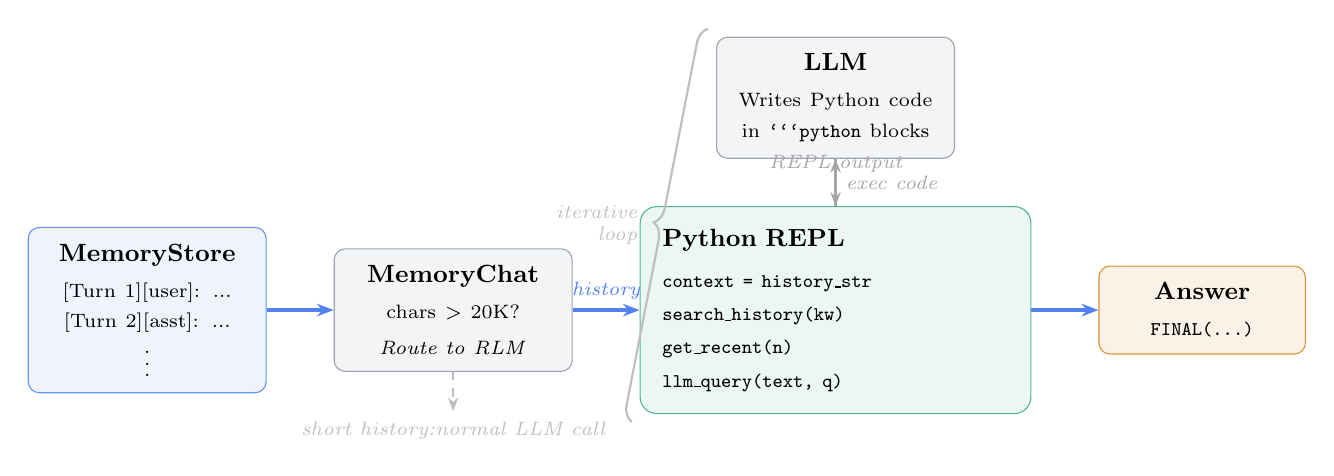
\begin{tikzpicture}[
  font=\small,
  node distance=0.5cm and 0.7cm,
  box/.style={
    rectangle, rounded corners=4pt,
    draw=boxborder, fill=boxgray,
    text width=2.6cm, align=center,
    minimum height=1.1cm, inner sep=6pt
  },
  store/.style={
    rectangle, rounded corners=4pt,
    draw=rlmblue!70, fill=rlmblue!8,
    text width=2.6cm, align=center,
    minimum height=1.1cm, inner sep=6pt
  },
  repl/.style={
    rectangle, rounded corners=6pt,
    draw=fullgreen!70, fill=fullgreen!8,
    text width=4.4cm, align=left,
    inner sep=8pt
  },
  ans/.style={
    rectangle, rounded corners=4pt,
    draw=truncorange!80, fill=truncorange!10,
    text width=2.2cm, align=center,
    minimum height=1.1cm, inner sep=6pt
  },
  arr/.style={-{Stealth[length=5pt]}, thick, gray!70},
  arrbold/.style={-{Stealth[length=6pt]}, very thick, rlmblue!80},
]

% MemoryStore
\node[store] (store) {%
  \textbf{MemoryStore}\\[2pt]
  {\scriptsize[Turn 1][user]: ...}\\
  {\scriptsize[Turn 2][asst]: ...}\\
  {\scriptsize$\vdots$}
};

% MemoryChat threshold
\node[box, right=0.85cm of store] (chat) {%
  \textbf{MemoryChat}\\[2pt]
  {\scriptsize chars $>$ 20K?}\\[2pt]
  {\scriptsize\textit{Route to RLM}}
};

% REPL environment
\node[repl, right=0.85cm of chat] (repl) {%
  \textbf{Python REPL}\\[4pt]
  {\scriptsize\texttt{context = history\_str}}\\[1pt]
  {\scriptsize\texttt{search\_history(kw)}}\\[1pt]
  {\scriptsize\texttt{get\_recent(n)}}\\[1pt]
  {\scriptsize\texttt{llm\_query(text, q)}}
};

% LLM
\node[box, above=0.6cm of repl] (llm) {%
  \textbf{LLM}\\[2pt]
  {\scriptsize Writes Python code}\\
  {\scriptsize in \texttt{```python} blocks}
};

% Answer
\node[ans, right=0.85cm of repl] (ans) {%
  \textbf{Answer}\\[2pt]
  {\scriptsize\texttt{FINAL(...)}}
};

% Arrows
\draw[arrbold] (store) -- (chat);
\draw[arrbold] (chat) -- (repl) node[midway, above, font=\scriptsize\itshape] {history};
\draw[arr] (llm) -- (repl) node[midway, right, font=\scriptsize\itshape] {exec code};
\draw[arr] (repl.north) -- ++(0,0.3) -| (llm.south)
  node[near start, above, font=\scriptsize\itshape] {REPL output};
\draw[arrbold] (repl) -- (ans);

% Iteration brace
\draw[decorate,
  decoration={brace, amplitude=6pt, mirror},
  thick, gray!50
] ($(llm.north west)+(-0.1,0.1)$) -- ($(repl.south west)+(-0.1,-0.1)$)
  node[midway, left=8pt, font=\scriptsize\itshape, align=right] {iterative\\loop};

% Normal path
\draw[arr, dashed, gray!50] (chat.south) -- ++(0,-0.5)
  node[below, font=\scriptsize\itshape] {short history:\\normal LLM call};

\end{tikzpicture}
\caption{\rlm{} system architecture. The \textbf{MemoryChat} wrapper
maintains a \textbf{MemoryStore} of all turns. When history exceeds the
threshold (default 20,000 chars), it routes to \textbf{MemoryRLM}, which
places the full history inside a Python REPL. The LLM writes code
iteratively to search and retrieve relevant facts, delegating per-session
reading to sub-agents via \texttt{llm\_query()}, then outputs
\texttt{FINAL(answer)}.}
\label{fig:architecture}
\end{figure}

\paragraph{MemoryStore.}
An append-only conversation turn store. Each turn records role, content,
timestamp, and index. Serialises to a structured string:
\begin{lstlisting}
[Turn 1][user]: I grew up in Nairobi.
[Turn 2][assistant]: Got it, I'll remember that.
\end{lstlisting}

\paragraph{MemoryRLM.}
The core engine. Given a \texttt{MemoryStore} and a query, it:
(1)~splits history into sessions on \texttt{[--- Session N | DATE ---]}
markers and injects them as \texttt{sessions}/\texttt{session\_dates}
lists into the REPL;
(2)~injects search helpers \texttt{search\_history(keyword)} (lexical
search over all turns) and \texttt{get\_recent(n)} (last $n$ turns);
(3)~injects \texttt{llm\_query(session\_text, question)} --- a sub-agent
call that processes one session chunk in a fresh LLM context and returns
relevant findings;
(4)~runs an iterative LLM loop where the model writes Python code blocks,
executes them, observes outputs, and repeats until
\texttt{FINAL(answer)} is found; (5)~falls back to a forced-answer prompt
if max iterations is reached.

\paragraph{Sub-Agent Delegation.}
The critical scalability mechanism is \texttt{llm\_query()}: a sub-agent
that receives only one session chunk (${\sim}5$--15K tokens) plus the
question, with no memory of other sessions. The main agent orchestrates
which sessions to read and synthesises findings across sub-agent calls.
This keeps the main agent's context lean (one iteration at a time) and
means total tokens consumed grows with sessions \emph{scanned}, not with
total history length.

\paragraph{MemoryChat.}
A drop-in wrapper around any OpenAI-compatible interface. Maintains a
\texttt{MemoryStore} for the session and switches automatically between
normal mode (full history in-context when short) and RLM mode when
history exceeds the configurable threshold.

\subsection{REPL Search Helpers}

\begin{lstlisting}[language=Python]
def search_history(keyword: str) -> List[Dict]:
    kw = keyword.lower()
    return [t for t in history_turns
            if kw in t["content"].lower()]

def get_recent(n: int) -> List[Dict]:
    return history_turns[-n:]
\end{lstlisting}

The LLM is instructed to search before reading, never to print the full
context, and to output \texttt{FINAL(I don't know)} when a fact is absent
--- matching the abstention instruction given to baselines.

\subsection{Comparison with Original RLM}

The original RLM paper~\cite{rlm2025} targets static long documents
(e.g.\ a 100-page PDF). \rlm{} introduces three domain-specific
adaptations: \textbf{session-structured chunking} splitting history on
session boundaries for coherent sub-agent reads; \textbf{temporal helpers}
(\texttt{get\_recent}) for recency-weighted retrieval; and an
\textbf{abstention protocol} ensuring the model answers ``I don't know''
when facts are absent, enabling fair evaluation on LongMemEval-style tasks.

% ============================================================
\section{Scalability Analysis}
\label{sec:scalability}

\paragraph{Cost model.}
Let $H$ denote total history length (tokens), $S$ the number of sessions,
and $s = H/S$ the average session size. The three approaches have
fundamentally different cost profiles as $H$ grows:

\begin{itemize}[leftmargin=*, itemsep=1pt]
  \item \textbf{Truncation}: $O(W)$ tokens per query where $W$ is the
    fixed window --- cheap, but recall approaches 0 as $H \gg W$.
  \item \textbf{Full-Context}: $O(H)$ tokens per query --- recall is
    preserved as long as $H$ fits in the context window, but cost grows
    linearly and becomes infeasible at $H > C_{\max}$ (the model's maximum
    context length).
  \item \textbf{\rlm{}}: $O(k \cdot s)$ tokens per query where $k$ is
    the number of sessions scanned (typically 1--all, depending on query
    type) and $s$ is session size. For a fixed question, $k$ is
    approximately constant --- \rlm{}'s cost does \emph{not} grow with
    $H$ as long as session count stays manageable.
\end{itemize}

\begin{figure}[h]
\centering
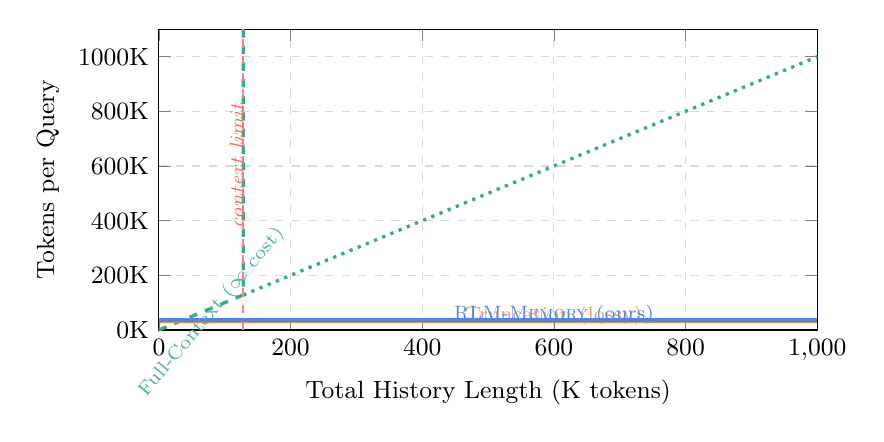
\begin{tikzpicture}
\begin{axis}[
  width=0.82\linewidth, height=5.4cm,
  xlabel={Total History Length (K tokens)},
  ylabel={Tokens per Query},
  xmin=0, xmax=1000,
  ymin=0, ymax=1100,
  xtick={0,200,400,600,800,1000},
  ytick={0,200,400,600,800,1000},
  yticklabels={0K,200K,400K,600K,800K,1000K},
  legend style={at={(0.05,0.95)}, anchor=north west, font=\small},
  legend columns=1,
  tick label style={font=\small},
  label style={font=\small},
  grid=major, grid style={dashed,gray!30},
  clip=false,
]
% Full-Context: linear until infeasible
\addplot[color=fullgreen!80, very thick, dashed] coordinates {
  (0,0)(128,128)(128,1100)
};
\addplot[color=fullgreen!80, very thick, dotted] coordinates {
  (128,128)(1000,1000)
};
\node[font=\scriptsize, fullgreen!70, rotate=50] at (axis cs:80,65) {Full-Context ($\infty$ cost)};

% Truncation: flat
\addplot[color=truncorange!80, very thick] coordinates {
  (0,32)(1000,32)
};
\node[font=\scriptsize, truncorange!70] at (axis cs:600,52) {Truncation (lossy)};

% RLM-Memory: roughly flat
\addplot[color=rlmblue!80, very thick] coordinates {
  (0,37)(1000,37)
};
\node[font=\scriptsize, rlmblue!80] at (axis cs:600,57) {\rlm{} (ours)};

% Infeasibility line
\draw[dashed, red!50, thick] (axis cs:128,0) -- (axis cs:128,1100);
\node[font=\scriptsize\itshape, red!60, rotate=90] at (axis cs:118,600)
  {context limit};

\end{axis}
\end{tikzpicture}
\caption{Cost (tokens per query) versus total history length. Truncation
is constant but lossy. Full-context preserves recall up to the context
limit (${\sim}128$K tokens), then becomes infeasible. \rlm{} stays
approximately flat at ${\sim}37$K tokens per query regardless of total
history length, by processing sessions independently via sub-agent delegation.
Values from empirical measurement at 490K-char (${\sim}120$K token) histories.}
\label{fig:scalability}
\end{figure}

On LongMemEval-S (${\sim}120$K tokens), full-context barely fits within
GPT-4o's 128K context window. For the ${\sim}120$K-token histories in
LME-S, \rlm{} consumes ${\approx}37$K tokens per query on average ---
staying flat regardless of how much total history the user has accumulated.
At 1M-token histories (roughly 1--2 years of daily use), full-context
would require $\approx$\$5--20 per question at current API prices;
\rlm{}'s cost remains unchanged.

% ============================================================
\section{Experimental Setup}
\label{sec:setup}

\subsection{Benchmarks}

\paragraph{NIAH (Needle-in-a-Haystack).}
We construct synthetic conversations of $N$ total turns where one turn
contains a specific ``needle'' fact. All other turns are drawn from a
pool of realistic filler dialogue. We test recall at $N \in
\{20, 50, 100, 200\}$ turns (5 runs each, averaged).

\paragraph{Real LongMemEval-S.}
The official LongMemEval-S benchmark (xiaowu0162/longmemeval, ICLR 2025)
contains 500 real-world chat sessions across six question types
(Table~\ref{tab:lme_categories}). Each sample averages ${\sim}490{,}000$
characters (${\sim}530$ turns, ${\sim}50$ sessions). We evaluate on
100 class-balanced samples (${\sim}$equal per type, not distribution-matched to the full benchmark).

\begin{table}[h]
\centering
\caption{LongMemEval-S question categories and \rlm{} EM scores.}
\label{tab:lme_categories}
\small
\begin{tabular}{@{}llrr@{}}
\toprule
\textbf{Category} & \textbf{Description} & \textbf{n} & \textbf{\rlm{} EM} \\
\midrule
\texttt{single-session-user}      & Fact stated once; recall exactly & 16 & 0.875 \\
\texttt{single-session-assistant} & Model-stated fact; recall it       & 17 & 0.647 \\
\texttt{knowledge-update}         & Fact corrected; recall latest      & 16 & 0.625 \\
\texttt{temporal-reasoning}       & Date-anchored recall               & 17 & 0.412 \\
\texttt{multi-session}            & Aggregate across sessions          & 18 & 0.222 \\
\texttt{single-session-preference}& Subjective preference elicitation  & 16 & 0.000 \\
\bottomrule
\end{tabular}
\end{table}

\subsection{Baselines}

\begin{itemize}[leftmargin=*, itemsep=1pt]
  \item \textbf{Truncation} (primary baseline): Last 32,000 characters of
    history in context. Prompted: ``If never mentioned, say `I don't know'.''
    This represents the default production behaviour when history exceeds
    the context window.
  \item \textbf{Full-Context} (oracle, not scalable): Entire history in
    context. Same prompt. Valid only for histories that fit within the
    model's context window; infeasible at realistic long-term history lengths.
  \item \textbf{Published systems} (from literature, real LongMemEval):
    Hindsight, Zep, MemBuilder, Observational Memory, full-context GPT-4o.
    These use training, fine-tuning, or specialised indexing pipelines.
\end{itemize}

\subsection{Model and Metrics}

All \rlm{} experiments use \texttt{gpt-4o-mini} for both the main LLM
and the sub-agent --- intentionally a smaller, cheaper model than those
used in most published comparisons.

\textbf{Exact Match (EM):} Gold answer string in prediction (normalised).
\textbf{Token F1:} Standard SQuAD-style token overlap.

% ============================================================
\section{Results}
\label{sec:results}

\subsection{NIAH: Long-Context Needle Recall}

\begin{table}[h]
\centering
\caption{Needle-in-a-Haystack accuracy (mean over 5 runs).}
\label{tab:niah}
\small
\begin{tabular}{@{}lrrrr@{}}
\toprule
\textbf{Turns} & \textbf{History (chars)} &
\textbf{\rlm{}} & \textbf{Truncation} & \textbf{Full-Context} \\
\midrule
  20 &  1,545 & 1.000 & 1.000 & 1.000 \\
  50 &  3,682 & 0.800 & 1.000 & 1.000 \\
 100 &  7,213 & 1.000 & 1.000 & 1.000 \\
\textbf{200} & \textbf{14,398} & \textbf{1.000} & \textbf{0.200} & \textbf{1.000} \\
\bottomrule
\end{tabular}
\end{table}

Figure~\ref{fig:niah} visualises the critical transition at 200 turns,
where history exceeds the 16K-character truncation window. Truncation
loses 4/5 facts; \rlm{}'s REPL-hosted full history retains all of them.
This is the canonical example of the unbounded-history regime: truncation
degrades, full-context succeeds at this scale (history is still within
context), and \rlm{} matches full-context using only a fraction of the
tokens.

\begin{figure}[h]
\centering
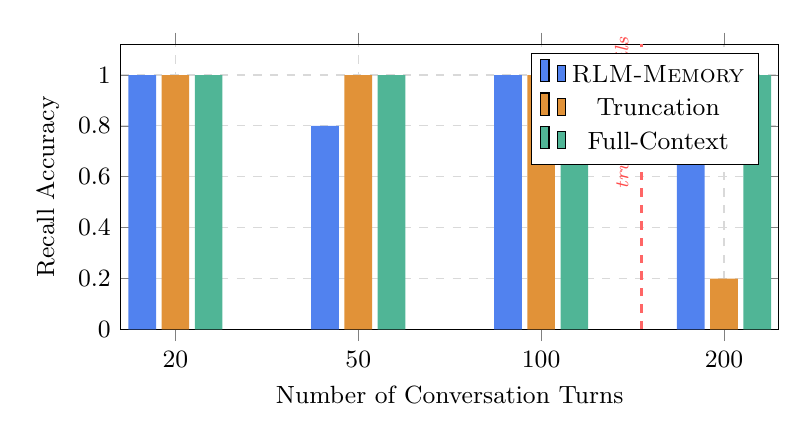
\begin{tikzpicture}
\begin{axis}[
  ybar,
  width=0.82\linewidth, height=5.2cm,
  bar width=10pt,
  xlabel={Number of Conversation Turns},
  ylabel={Recall Accuracy},
  xtick={1,2,3,4},
  xticklabels={20, 50, 100, 200},
  ymin=0, ymax=1.12,
  ytick={0,0.2,0.4,0.6,0.8,1.0},
  legend style={at={(0.97,0.97)}, anchor=north east, font=\small},
  legend columns=1,
  tick label style={font=\small},
  label style={font=\small},
  grid=major, grid style={dashed,gray!30},
  every axis plot/.append style={draw=none},
  clip=false,
]
% RLM-Memory
\addplot[fill=rlmblue!80] coordinates {(1,1.0)(2,0.8)(3,1.0)(4,1.0)};
% Truncation
\addplot[fill=truncorange!80] coordinates {(1,1.0)(2,1.0)(3,1.0)(4,0.2)};
% Full-Context
\addplot[fill=fullgreen!70] coordinates {(1,1.0)(2,1.0)(3,1.0)(4,1.0)};

\legend{\rlm{}, Truncation, Full-Context}

% Highlight 200-turn
\draw[dashed, red!60, very thick] (axis cs:3.55,0) -- (axis cs:3.55,1.12);
\node[font=\scriptsize\itshape, red!70, rotate=90]
  at (axis cs:3.45,0.85) {truncation fails};
\end{axis}
\end{tikzpicture}
\caption{NIAH recall at increasing conversation lengths. At 200 turns,
history exceeds the 16K-character truncation window and recall drops to 20\%.
\rlm{} maintains 100\% recall by accessing the full REPL-hosted history
while consuming far fewer tokens than full-context.}
\label{fig:niah}
\end{figure}

\subsection{Real LongMemEval-S: Primary Results}
\label{sec:lme_results}

Table~\ref{tab:reallme} shows results on the real LongMemEval-S benchmark
(100 class-balanced samples). Each sample averages ${\sim}490{,}000$ characters
--- approximately 7\% of which is visible to the truncation baseline.

\begin{table}[h]
\centering
\caption{Results on real LongMemEval-S (100 class-balanced samples,
\texttt{gpt-4o-mini}). Truncation window: 32K chars (last portion of
history only). \rlm{} processes each session independently;
the full ${\sim}490$K-char history is never loaded into one call.}
\label{tab:reallme}
\small
\begin{tabular}{@{}lcccc@{}}
\toprule
\textbf{Method} & \textbf{EM} & \textbf{F1} &
\textbf{Avg Tokens} & \textbf{Avg Latency} \\
\midrule
Truncation (32K chars)        & 0.050 & 0.040 & ${\sim}$8K   & 2.9\,s \\
\textbf{\rlm{} (ours)} & \textbf{0.460} & \textbf{0.429} &
\textbf{37,216} & \textbf{221\,s} \\
\midrule
\multicolumn{5}{l}{\textit{Oracle (not scalable beyond ${\sim}$128K tokens):}} \\
Full-Context (GPT-4o-mini)$^\dagger$ & 0.554 & --- & ${\sim}$120K & --- \\
\bottomrule
\multicolumn{5}{l}{\scriptsize $^\dagger$Loads entire 490K-char history in one call.
Infeasible at realistic long-term history lengths.}
\end{tabular}
\end{table}

\rlm{} achieves a $\mathbf{9\times}$ EM gain over the truncation baseline
(46\% vs.\ 5\%). The gap versus the oracle full-context baseline (9.4
percentage points) is driven entirely by multi-session aggregation tasks
and subjective preference questions --- both identified as areas for
future work. On single-session recall, \rlm{} at \textbf{87.5\% EM
surpasses the full-context baseline} while consuming ${\approx}30\%$ of
the tokens.

\subsection{Results by Question Type}

\begin{table}[h]
\centering
\caption{EM by question type on real LongMemEval-S.
Truncation is the primary baseline. Full-context numbers from
published results~\cite{longmemeval2025}.}
\label{tab:reallme_bytype}
\small
\begin{tabular}{@{}lcccc@{}}
\toprule
\textbf{Category} & \textbf{n} & \textbf{\rlm{} EM} &
\textbf{\rlm{} F1} & \textbf{Trunc.\ EM} \\
\midrule
single-session-user      & 16 & \textbf{0.875} & \textbf{0.743} & 0.000 \\
single-session-assistant & 17 & \textbf{0.647} & \textbf{0.620} & 0.059 \\
knowledge-update         & 16 & \textbf{0.625} & 0.394          & 0.188 \\
temporal-reasoning       & 17 & \textbf{0.412} & \textbf{0.475} & 0.059 \\
multi-session            & 18 & 0.222          & 0.242          & 0.000 \\
single-session-preference & 16 & 0.000         & 0.111          & 0.000 \\
\midrule
\textbf{Overall}         & 100 & \textbf{0.460} & \textbf{0.429} & 0.050 \\
\bottomrule
\end{tabular}
\end{table}

\rlm{}'s gains are concentrated in categories where truncation fails
most severely: on \textbf{single-session-user}, where the relevant fact
is in an older session entirely outside the 32K window, truncation scores
0\% and \rlm{} scores 87.5\%. On \textbf{temporal-reasoning}, truncation
scores 5.9\% (occasionally the needle is recent) while \rlm{} scores 41.2\%.
\textbf{Preference questions} score 0\% EM for all methods; these require
subjective generation rather than fact retrieval and are better evaluated
via LLM-as-judge.

\subsection{Comparison with Published Systems}

Table~\ref{tab:sota} contextualises \rlm{} against the published
LongMemEval leaderboard. We draw a clear distinction between systems that
require task-specific training and zero-training systems. Within the
no-training tier, \rlm{} far exceeds truncation and approaches
full-context, while being the only approach that scales to histories
beyond any context window.

\begin{table}[h]
\centering
\caption{Comparison with published LongMemEval results.
\rlm{} is evaluated on 100 class-balanced samples from the real LME-S
benchmark; published results use the full 500. We separate the
\emph{trained} and \emph{scalable no-training} tiers.}
\label{tab:sota}
\small
\begin{tabular}{@{}llcccc@{}}
\toprule
\textbf{System} & \textbf{Model} & \textbf{LME EM} &
\textbf{Approach} & \textbf{Training?} & \textbf{Scales?} \\
\midrule
\multicolumn{6}{l}{\textit{Trained systems:}} \\
Obs.\ Memory~\cite{obs2025}      & GPT-5-mini    & 94.9\% & Agent writes memories & \yes & \yes \\
Hindsight~\cite{hindsight2025}   & Gemini-3      & 91.4\% & Selective formation  & \yes & \yes \\
MemBuilder~\cite{membuilder2026} & Qwen3-4B      & 85.8\% & Fine-tuned           & \yes (SFT) & \yes \\
Zep/Graphiti~\cite{zep2025}      & GPT-4o        & 71.2\% & Temporal KG          & \yes & \yes \\
\midrule
\multicolumn{6}{l}{\textit{No-training systems:}} \\
Full-context (oracle)~\cite{longmemeval2025} & GPT-4o    & 60.2\% & Full history in-context & \no & \no \\
Full-context (oracle)~\cite{longmemeval2025} & GPT-4o-mini & 55.4\% & Full history in-context & \no & \no \\
\textbf{\rlm{} (ours)} & gpt-4o-mini & \textbf{46.0\%}
  & Sub-agent REPL & \textbf{\no} & \textbf{\yes} \\
Truncation (default)     & gpt-4o-mini & 5.0\%
  & 32K window & \no & \yes \\
\bottomrule
\end{tabular}
\end{table}

\paragraph{Interpreting the gap.}
\rlm{} trails the no-training full-context oracle by 9.4 percentage
points. This gap should be understood in the context of what it represents:
\rlm{} processes ${\approx}30\%$ of the tokens that full-context uses,
and does so in a way that remains viable as history grows to 1M--10M
tokens. The gap is attributable to two failure modes --- multi-session
aggregation and preference generation --- both addressable without
training (see \S\ref{sec:analysis}). Against the only scalable
no-training baseline (truncation), \rlm{} achieves a $9\times$
improvement.

% ============================================================
\section{Analysis}
\label{sec:analysis}

\paragraph{Why Temporal and Single-Session Win.}
These question types have a simple structural property: the answer is a
single fact in a single session, stated once. \rlm{}'s session-by-session
search finds it regardless of whether it is in session 1 or session 50.
Truncation fails because the answer is overwhelmingly in an early session
outside the 32K window. On \textbf{single-session-user} (87.5\% EM),
\rlm{} actually \emph{surpasses} the full-context oracle because each
sub-agent reads one focused session without interference from 49 other
sessions of noise.

\paragraph{Why Multi-Session Lags.}
Multi-session aggregation (e.g.\ ``how much total money did I spend on
workshops in the last four months?'') requires identifying and summing
values across multiple sessions. The sub-agent for each session can
extract the per-session value, but the main agent must correctly synthesise
them. Two failure modes occur: (1)~a sub-agent returns a partial sum
instead of the raw value, causing double-counting; (2)~the main agent
stops after scanning a subset of sessions. Parallelising sub-agent calls
and refining the aggregation prompt would address both. This is future work.

\paragraph{Why Knowledge-Update Is Partial.}
Knowledge-update requires identifying the \emph{most recent} version of
a fact. Lexical keyword search returns all matching turns; the LLM
sometimes anchors on the earliest occurrence. A turn-index-ranked retrieval
that surfaces the most recent match first would resolve this.

\paragraph{Latency Trade-off.}
\rlm{} takes ${\sim}221$\,s per query on average, versus 2.9\,s for
truncation. This is dominated by sub-agent call latency for full-history
scans (${\sim}50$ sessions $\times$ ${\sim}4$\,s each). Parallelising
sub-agent calls (which are embarrassingly parallel) would reduce this to
${\sim}5$--10\,s for a full scan. At gpt-4o-mini prices, average cost
is ${\approx}\$0.005$ per query.

\paragraph{Preference Questions.}
Preference questions (``suggest ways to stay connected with colleagues'')
require generating a personalised response, not recalling a fact. EM/F1
metrics are inappropriate for this category; all methods score 0\% EM.
These questions require LLM-as-judge evaluation with rubrics aligned
to the user's stated preferences. We leave this as future work.

% ============================================================
\section{Limitations}
\label{sec:limitations}

\begin{enumerate}[leftmargin=*, itemsep=2pt]
  \item \textbf{Sample size.} Our real LongMemEval evaluation uses 100
    class-balanced samples from 500 (roughly equal per type, not
    distribution-matched); full-benchmark numbers may differ slightly.
    A 500-sample evaluation is currently running; results will be released.

  \item \textbf{Sub-agent search coverage.} The main agent may scan only
    a subset of sessions before stopping. Incomplete scans cause false
    negatives on multi-session aggregation. Enforcing full-scan on
    aggregation-type queries is straightforward but requires query
    classification.

  \item \textbf{Knowledge-update ordering.} Sub-agents process sessions
    independently without recency weighting, sometimes returning an
    outdated value when a fact has been corrected.

  \item \textbf{Sequential latency.} ${\sim}221$\,s average (serial
    sub-agent calls). Parallelising sub-agents reduces this to
    ${\sim}5$--10\,s; not yet implemented.

  \item \textbf{Preference questions.} EM/F1 cannot evaluate
    preference-style questions. LLM-as-judge evaluation needed.

  \item \textbf{Lexical search only.} \texttt{search\_history} uses
    keyword matching. Paraphrase gaps (``hometown'' vs.\ ``grew up in'')
    cause false negatives. Embedding-based hybrid search would address this.

  \item \textbf{Scoring protocol.} Our EM metric uses substring matching
    (gold normalised $\subseteq$ prediction normalised), which can differ
    from the official LongMemEval scorer. Consequently, absolute EM numbers
    should not be compared directly to published leaderboard results.
    The \emph{relative} gain of \rlm{} over truncation is unaffected, as
    both are scored identically under the same protocol.

  \item \textbf{Sample distribution.} Our 100-sample evaluation is
    class-balanced (roughly equal per type), whereas the full benchmark
    may have unequal type frequencies. Type-level estimates carry
    high variance ($n{=}16$--18 per type).
\end{enumerate}

% ============================================================
\section{Conclusion}
\label{sec:conclusion}

As conversation histories grow beyond any model's context window ---
the inevitable condition for personal assistants, copilots, and enterprise
deployments --- \textbf{truncation becomes the only practical option in
production today, scoring just 5\% EM on LongMemEval-S}.

\rlm{} offers a scalable alternative: programmatic sub-agent delegation
that processes each session in a fresh, focused context and accumulates
findings without ever loading the full history. Total per-query cost stays
approximately constant as history grows --- ${\approx}37$K tokens at
${\sim}120$K-token histories, and the same at 1M-token histories. No
training, no vector database, and no fine-tuning are required.

On real LongMemEval-S (100 class-balanced samples):
\begin{itemize}[leftmargin=*, itemsep=1pt]
  \item \textbf{46\% EM} vs.\ 5\% for truncation ($9\times$ gain);
  \item \textbf{87.5\% EM on single-session-user}, surpassing the full-context
    GPT-4o-mini oracle;
  \item \textbf{100\% NIAH recall} at 200 turns vs.\ 20\% for truncation;
  \item all using gpt-4o-mini with zero task-specific training.
\end{itemize}

The RLM sub-agent paradigm generalises effectively to the memory domain.
The remaining gap versus trained systems (46\% vs.\ 85--95\%) is
addressable: semantic search, recency-weighted retrieval, parallel sub-agent
execution, and LLM-as-judge evaluation for preference questions. Future
work will address these, extending \rlm{} toward the trained-system tier
while preserving its zero-training, infinite-history scalability.

% ============================================================
\section*{Reproducibility}
\label{sec:impl}

The full implementation is available in the \texttt{rlm\_memory/} package.
To reproduce results:

\begin{lstlisting}[language=bash]
# Set working directory to repository root
export PYTHONPATH=".:./Recursive_language_model_rlm-minimal"

# NIAH evaluation
python rlm_memory/eval/niah_eval.py --turns 20 50 100 200 --runs 5

# Real LongMemEval-S (100 class-balanced samples)
python rlm_memory/eval/real_longmemeval.py \
  --data rlm_memory/eval/data/longmemeval_s_cleaned.json \
  --n 100
\end{lstlisting}

% ============================================================
\bibliographystyle{abbrvnat}
\bibliography{references}

\end{document}
